\documentclass[a4paper,11pt]{kth-mag}

\usepackage[T1]{fontenc}
\usepackage{amsfonts}
\usepackage{textcomp}
\usepackage{graphicx}
\usepackage{array}
\usepackage{pbox}
\usepackage{hyperref}
\usepackage{lmodern}
\usepackage[utf8]{inputenc}
\usepackage[swedish,english]{babel}
\usepackage{nada-ex}
\usepackage{subcaption}
\usepackage[backend=biber]{biblatex}
\usepackage{csquotes}
\usepackage{tikz}
\usepackage{color, colortbl}

\def\arraystretch{1.5}

\definecolor{LightGray}{gray}{0.93}
\definecolor{Gray}{gray}{0.83}

\addbibresource{ressources.bib}

\graphicspath{{img/}}

\title{Inside the Black Box: How to Explain Individual Predictions of a Machine Learning Model}
\subtitle{How to automatically generate insights on predictive model outputs, and gain 
	a better understanding on how the model predicts each individual data point.}
\author{Marc Beillevaire}
\date{December 2016}
\blurb{
	Master's Thesis at CSC \\
	Supervisor: Hedvig Kjellström \\
	Examiner: Danica Kragic
}
\trita{TRITA xxx yyyy-nn}
\begin{document}
\frontmatter
\maketitle


\begin{abstract}
Machine learning models are becoming more and more powerful and accurate, but their good predictions usually come with a high complexity. Depending on the situation, such a lack of interpretability can be an important and blocking issue. This is especially the case when trust is needed on the user side in order to take a decision based on the model prediction.

In this thesis, several explanation methods are described and compared on multiple datasets (text data, numerical), on classification and regression problems.
\end{abstract}

\clearpage
\selectlanguage{swedish}
\begin{abstract}
på svenska

jag tycker om kannelbullar
\end{abstract}
\selectlanguage{english}
\clearpage
\tableofcontents
\mainmatter



\chapter{Introduction}

This first chapter is an introduction to the problem raised in this master thesis and provides an overview on how it is structured. It first describes the backgrounds and motivations for this project, and set the research question as well as a high-level view on the methodology and the approach chosen to deal with it.

\section{Background}

This project has been conducted at \textit{Dataiku}, in Paris. Dataiku is a young startup developping \textit{Dataiku DSS} -- standing for Data Science Studio. This software is a collaborative plateform on which data scientists and data analysts can easily perform data processing operations, such as: collecting the data, cleaning it and doing some preprocessing, training and applying machine learning algorithms as well as putting a process into production in a few clics.

Besides developping Dataiku DSS, the company also helps companies to set up data science projects by providing both the technical solutions and the scientific expertise from Dataiku's data scientist team. Today, their customers are spread out around the world. After securing a series A fundraising in October 2016, the company's next goal is to appear among the top data science plateforms in the USA anytime soon.

This project was initiated after several feedbacks from Dataiku customers. They are always looking for more trust and transparence towards the models they are using, and this is one of the key issues when machine learning models are required for taking actions in a company. Thus, Dataiku's customers are often asking for more insights, and many of them especially want to know why such a prediction has been made by a given model, on a given data point.

This projects aims at providing a selection of practical solutions to this problem to the Dataiku team. The purpose is also to make their use simple by providing Dataiku DSS plugins, as well as webapps for visualization purposes.

\section{Motivation}

Predictive models using machine learning are getting more and more efficient while spreading in many areas in both industrial and services companies. Many companies are collecting and using their own data more and more to optimize various processes. For instance, in online marketplaces customers' data are constantly processed by machine learning algorithms, whether it is for recommendation or to track potential fraudsters.

Yet, while most companies are eager to set up very efficient predictive models, a strong limitation still holds: when a human decision maker has to take an action \textit{according to a prediction made by a model}, trust in the model becomes at least as important as the accuracy of the prediction itself. People cannot willingly accept to take a decision just because a computer said so, and they need to be provided with insights and explanations on why the model produced a given output. This is why the demand for new insights at the prediction level is important: global coefficients at the model level are not enough, most of the time the real question is \textit{"Why this model made such a prediction ?"}.

This is the case in many areas: in fraud detection on an e-commerce website,  taking an action could mean adding another layer of security during a purchase like 3D security, which decreases the user experience and could lead to fewer purchases. With predictive maintenance models, maintenance operations on the equipment costs money, and such a predictive model would be used by decision makers \textit{only} if they believe the algorithm can effectively predict the next failures of the equipment. Hence how efficient such models may be, they would only be applied if the business owners trusts them to effectively optimize the company's processes.

This necessity for insights is going to be more significant in the years to come in the European Union. Indeed in April 2016, the European Parliament adopted \href{http://eur-lex.europa.eu/eli/reg/2016/679/oj}{the General Data Protection Regulation (GDPR)}. Besides new rules regarding data protection, it provides every European citizen a \textit{right to explanation} \cite{euregulation}: every decision having an impact on someone's life will have to be motivated by an explanation, even when the decision is taken by an algorithm. For instance, a bank agency will not be able to refuse a loan based only on an algorithmic decision.

\section{What information should an explanation bring ?}
% Titre ok ??

The main purpose of individual explanations is to bring \textit{trust} to users of machine learning models. According to some articles, interpretability is a prerequisite for \textit{trust} \cite{lime} \cite{mythos}. Trust could actually be assessed by a simple score of the model, but it usually requires more than that: users are generally more comfortable when they understand the models they trained. Moreover, one can trust a model to be efficient, but not to respect some criteria and constrainsts such as ethics or legality \cite{mythos}.

Therefore, an explanation algorithm must ensure understandability in each predictions that are explained. This mean producing an output that is easy to read and interpret for a human being, and that relies on the users' previous knowledge on the data in order to help them understand the model's behaviour.

This leads to the following remarks: an explanation should be kept short, so that it is immediately fully understood by the user. For instance: a linear model, even easily interpretable by nature, will not be understood if there are several hundreds of variables. Besides, the user is supposed to have knowledge on the features in the dataset, so it is fine to use this in order to build explanations.

Therefore, in this thesis an explanation will consist on a short list of features, with a weight assigned to each of them.

\section{Problem statement and methodology}

The goal of this thesis is to test several algorithms that automatically extract explanations from the model and to assess their goodness to compare them.

These algorithms have two main purposes: effectively provide explanation for each prediction made by the model, and also assessing the goodness of the model. Indeed when looking at explanations, a user with prior knowledge on the data will be able to tell if the model relies on relevant features. If a model is trained and tested on a datasets where some features are falsly correlated to the output, then the model is probably not very good -- not generalizable on new data that does not provide these falsly correlated features.

For instance, assume an image classification model only sees the blue sky to detect airplanes. If there are only planes in the sky, its score will probably be high. But what if a bird flying in the sky is set as input ? The model has a high probability to classify it as a plane.

Using efficient explanations, this could be anticipated: the explanations for examples in the \textit{plane} class would show that only the blue sky matters to the model. Human beings can clearly see that the model did not detect the real object. Therefore they could assess that this model is not actually good at classifying planes, no matter how high its accuracy on the test set is.

In this project, this goodness measure will be used to test the explanations algorithm. The goal of the explanaining algorithm is to point out the wrong features that are used by bad models. So our methodology will be the following:

\begin{itemize}
	\item Set up two datasets: one with both useful and useless features, another one containing only the good features
	\item Train a model using the first dataset, test it on the second one
	\item Extract explanations from predictions on several examples
	\item Remove the bad features that popped up in the explanations, retrain the model
	\item Check if the score improved on the second model
\end{itemize}

Here, we expect the score on the second dataset to be quite low, because the model learned some wrong correlations between useless features and the target. If the explanations are relevant, they should point out the most important features that are used by the model on several examples. Using the prior knowledge on the features, the bad ones can be removed, and the score on the second (clean) set should improve.

\section{Framework}

Most of the time explanations algorithms can work with any type of model: either regression or classification models as long as they output probability for each class. We will focus on classic, widely-used algorithms such as linear models, Classification and regression trees \cite{cart}, Random Forests \cite{Breiman2001}, Gradient Boosted Trees \cite{Friedman2001}.

The type of data that will be considered will be tabular data sets (feature vectors with a target) as well as textual data. This is of course generalizable to any type of data, like image classification and neural networks, but to stick with reasonable amount of data and limited training time, these kind of datasets and methods will not be investigated.

The method will be tested on several datasets. Therefore the output will be changing, and an algorithm can be good to extract explanations on specific data while being less efficient on other datasets. Yet, we expect our methodology to show consistent results that should not vary too much between different datasets.

\section{Outline}

This thesis is divided into 5 chapters.

The \textit{Introduction} chapter provides the background and motivation for this project. The methodology is also stated, as well as the hypothesis for an explanation algorithm to be good enough. Finally the framework part provide information on the frame and the limitations of this thesis.

The \textit{Background} chapter focuses on the algorithms published in the litterature, where the most important papers in this field of research will be examined. This chapter will also cover the background knowledge needed for the rest of the thesis. Not so many papers are related to model explanations at the prediction level. Yet they nearly all propose a different approach to this issue.

The \textit{Method} chapter is dedicated to how the experiment will be performed. The datasets are specified, as well as the various models used for the tests. The technical content will be further described in this chapter. Especially, several algorithms that compute explanations on individual predictions will be provided. The metrics used to assess whether an algorithm is good or not to extract explanations is also further described here.

The \textit{Experiments} part describes the experiments conducted in this thesis. This chapter provides all the results obtained according to the method of the previous chapter.

Finally, the \textit{Discussions} chapter summarize the results and discuss the different methods explored here. This chapter also describe some limitations to this thesis, and provides potential improvements and what could be the future work on this topic.

\chapter{Background}

This chapter provides the technical background to this thesis. The litterature study show a relatively important interest in this field for the last decade, and a great variety of algorithms presented in research papers.

This chapter is divided in two parts as there are two main solutions for this problem of explaining individual models' predictions. Either the algorithm uses the inherant structure of the model to compute explanations like the tree structure for tree-based models. Or it considers the model as a black box and only uses the input-output matching that it produces.

The first type of algorithms will be called \textit{model-dependent} explanations algorithms, while the second type are denoted by either the term \textit{model-independant} or \textit{model-agnostic} explanations. Both these two solution have some advantages and drawbacks, and several implementations in these two categories will be investigated.

\section{Model-dependant explanations}

This first type of explanations implies for the explanations algorithm to understand how the explained model is build, making use of its particular type to extract explanations from it. A real advantage for these methods is that explanations are usually faster to compute. Yet, they suffer from not being generalizable to other types of models. Moreover two different model-dependent explanations cannot be compared if they has been computed on two different types of models.

\subsection{Linear models}

By definition linear models are easy to interpret without a complicated on-top explanations algorithm: one only has to look at the regression coefficients to see the relative importance of each variable.

The output of a linear model is the following:

\[
	P(x_1, ..., x_n) = f \left( \sum b_i x_i \right)
\]

where $(x_1, ..., x_n)$ is the current data point, and the values $(b_i)_{i \in [1, n]}$ are the coefficients of the linear model. The function $f$ maps the sum into the output space. For linear regression, $f$ is the identity function, while for logistic regression, $f$ is the sigmoid function: $f(x) = \frac1{1 + e^{-x}}$.

It is then easy to compute the contribution of the features to the outcome: as the output depends directly on the sum of the feature value multiplied by the regression coefficient, multiplying each regression coefficient by the feature value give the direct influence of the feature value on the prediction. Each term $b_i x_i$ represents therefore the influence of each feature to the output. In the case of linear regression, it is even the direct contribution to the output, but for logistic regression, the sigmoid function prevent from a meaningful comparison between each $b_i x_i$ and the predicted value.

\begin{figure}[!h]
	\centering
   	\def\svgwidth{\columnwidth}
	\includegraphics[scale=0.5]{linear_explanation.png}
    \caption{Feature contributions for a linear model.}
\end{figure}


The limit in interpretability of a linear model is only the dimension of the input space: if there are hundreds of features to consider, then another step is needed. It can simply be a list of the top $N$ coefficients, $N$ being small enough. But we could also consider a feature selection algorithm that keeps a small number of features before fitting the model.

The interesting thing in linear models is the ability to predict how the model will behave when moving the data point in the feature space. It only requires to look at the model coefficients: a positive coefficient means that increasing the feature increases the output, and vice-versa with negative coefficients. For interpretation purposes, this is very convenient: when users of a model can take actions to change the input variables, they know which ones to change in order to adapt the output.

\subsection{Tree-based models}

An explaining algorithm for tree-based models -- classification and regression trees, random forests and gradient boosted trees -- has been developed by \citeauthor{treeinterpreter} in a blogpost \cite{treeinterpreter}.


It works as follow: initially the contribution for each feature is set to 0. When computing predictions using a tree, the data point $x$ goes down in the tree, starting from the root, following a series of rules based on the features values. At each step down, the features space is split into two disjoint parts along one axis because only one feature is involved in one cut. The algorithm then computes for this cut the difference between the proportion of $\hat{y}$ -- the model output -- in the subspace where $x$ lies and the proportion of $\hat{y}$ in the bigger space.

This quantity is summed to the contribution of the feature involved in the cut. This value answers the question: at a given step, how well did the feature improve the classification of the example ?

To understand this process better, let's assume we have a train dataset of 2-dimentional points, a new example to classify, and that we use the following tree to classify the points into two classes:


\begin{figure}[h!]
\centering
\begin{subfigure}{.55\textwidth}
	\centering

	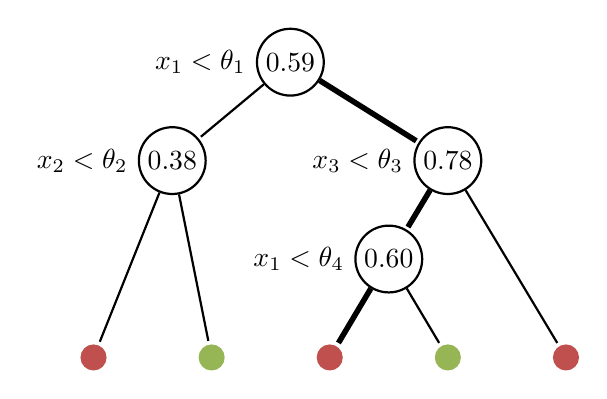
\begin{tikzpicture}[->,>=,shorten >=1pt,auto,thick,
    	 inner node/.style={circle,draw,inner sep=2pt},
    	 red node/.style={circle,fill=pastelred},
    	 green node/.style={circle,fill=pastelgreen}]

	\definecolor{pastelred}{RGB}{192,80,77}
	\definecolor{pastelgreen}{RGB}{150,182,86}

  	\draw (0,0)     node[inner node,label=left:$x_1 < \theta_1$] (1) {0.59};
	\draw (-1.5,-1.25) node[inner node,label=left:$x_2 < \theta_2$] (2) {0.38};
	\draw (2,-1.25)  node[inner node,label=left:$x_3 < \theta_3$] (3) {0.78};
	\draw (1.25,-2.5)    node[inner node,label=left:$x_1 < \theta_4$] (4) {0.60};
	
	\fill (-2.5,-3.75)   node[red node]   (5) {};
	\fill (-1,-3.75) node[green node] (6) {};
	\fill (0.5,-3.75)    node[red node]   (7) {};
	\fill (2,-3.75)  node[green node] (8) {};
	\fill (3.5,-3.75)    node[red node]   (9) {};
  	
  	\path[every node/.style={font=\sffamily\small}]
    (1) edge      (2) 
        edge[line width=2pt] (3)
    (2) edge      (5)
        edge      (6)
    (3) edge[line width=2pt] (4)
        edge      (9)
    (4) edge[line width=2pt] (7)
        edge      (8);
        
	\end{tikzpicture}
  
  \caption{A subfigure}
  \label{fig:sub1}
\end{subfigure}%
\begin{subfigure}{0.45\textwidth}
  \centering
  \includegraphics[width=1.0\linewidth]{img/decisiontree.png}
  \caption{A subfigure}
  \label{fig:sub2}
\end{subfigure}
\caption{A figure with two subfigures}
\label{fig:test}
\end{figure}

The green and red dots represent the training set, and the grey dot a new example to classify. At each node of the tree, a test is performed (Is $x_i$ smaller than $\theta_j$ ?) in order to drive the grey point either on the left or the right branch. The numbers on the nodes indicate the proportion of red dots in each subspace represented by this node. On the leafs, this proportion is either 0 or 100\% -- the leaf represents either a green subspace or a red subspace here.

The grey dot is the new example to classify. It will, of course, be classified as red by the classification tree, going through the bold path to the red leaf. 
Between the root and the second node encountered by the example while being classified, the feature $x_1$ is used, and the classification improves since the proportion of red points goes from 0.59 to 0.78. Hence, the contribution of feature $x_1$ is positive at this step and is increased by $0.78 - 0.59 = 0.19$.

Then feature $x_2$ is used, and this step reduces the proportion of red dots by $0.18$. Finally, feature $x_1$ is used again, increasing the probability from 0.60 to 1. 

Summing all the contributions along the path, the explanation for this classification are the following contributions towards class \textit{Red}:

\begin{center}
\begin{tabular}{|c|c|}
\hline
Feature $x_1$ & 0.59 \\
\hline
Feature $x_2$ & -0.18 \\
\hline
\end{tabular}
\end{center}

This solution is easily adaptable to ensemble methods using trees as their base model: contributions to each feature can be summed over all the trees, and average according to the importance of each tree in the classifier.

In the case of Random Forests, where all the trees are given the same weight, contribution for feature $i$ is computed as follow:
\[
	\mathrm{contrib}_i(x) = \sum_{tree t} \mathrm{contrib}_{t,i} (x)
\]

This way of exploring trees through the path of the original datapoint makes this algorithm efficient: its complexity is proportional to the height of the tree, and linear in the number of trees if the algorithm is an ensemble.

\section{Model-independent explanations}

Although model-dependent methods are computationally efficient, they still rely on specific models. A model-independent or model-agnostic algorithm would be preferable for at least two reasons: its ability to explain any type of classifiers and regressors, and the possibility to compare two explanations from two different model, even when these models are of different types.

Several algorithms has been developed, most notably: \cite{lime}, \cite{explvect}, \cite{ice}, \cite{gametheory}, \cite{documentclassif}. They nearly all develop a different approach to extract explanations from a specific prediction, albeit some similarities exist between some of them.

For some authors, the way to understand a prediction is to locally estimate the output of the model. That is, understand how the model behave around the data point of interest in the features space.

Thus, several solutions involve estimating the local output distribution from the model, like \textit{Lime} \cite{lime} and \citeauthor{explvect}'s \textit{explanation vectors} \cite{explvect}. If the model is a classifier that outputs probabilities, then the output distribution is a probability distribution in the feature space. 

\subsection{Lime: a local estimation by a simpler model}

\textit{Lime} algorithm \cite{lime}, standing for \textit{Locally Interpretable Model-agnostic Explanations}, is a recent solution proposed by \citeauthor{lime}. The authors' main idea is to locally estimate a complicated model by a simpler one that is interpretable. The goal is then to find a new model that is a good local estimator of the complex model, so the new model should be locally faithful to the original model.

Given the constrainst of interpretability, linear models are the first obvious choice to use as simple models. When a limited number of features is used, then such models become easily interpretable by humans. Simple decision trees that are not too deep could also make good interpretable models, but only linear models will be used here.

To locally approximate a model seen as a black box by a linear model, Lime's process is the following:

\begin{itemize}
	\item Sample $N$ points according the the training set distribution. Generally several thousands of points are needed so that Lime gets an accurate enough view of the training set.
	\item Apply the black box estimator to each of the sample. All these outputs will form the targets of the new training dataset.
	\item Weight each sample using a gaussian kernel centered on the point of interest
	\item Fit a linear model to the new dataset formed by the samples and the complicated model outputs.
\end{itemize}

\begin{figure}[!h]
	\centering
   	\def\svgwidth{\columnwidth}
	\includegraphics{lime-schema.png}
    \caption{Local estimation by a linear model around the bold red cross}
\end{figure}

In the author's implementation \cite{limeGitHub}, the sampling is made after \textit{discretizing the training set}: each feature is splitted in several parts using a binning method (quantiles, histograms, supervized binning). Then each new sample is generated feature by feature following this binning. This may not be the most accurate way to mimic the training distribution but it is fast --- linear in the number of features --- and lead to a very fast sampling. Furthermore, the goal is only to generate points in space, and the fact that some of them are distant from the initial point is not a problem since the gaussian kernel weighting (at step 3) will keep the linear model locally accurate: points that are far away will not be taken into account in the local model, while closer ones will be considered as most important.

In this thesis, we also tested a supervized binning: the bins along a given feature are created using the target values. This binning is based on entropy, meaning that at each step a split would minimize the entropy in the new bins. Such binning proves useful when data is not gaussian and very skewed: for instance, if more than 50\% of the points have value zero, then the first two quartiles consist only on these zero-value points. The entropy discretizer, on the contrary, will tend to explore more over the whole span of the data.

At Dataiku, a good usecase for this discretizer has been on \textit{fraud detection data} for an online seller. When focusing on the number of credit card used per user, one would notice that more than 80\% of the users only use 1 single credit card, and a very few, potential fraudsters, uses 10 or more. Quartile discretizer here would only split the data between "1 credit card" points and "at least 2 credit card" points, while the entropy discretizer will notice that most fraudsters used a lot of different credit cards, and make several splits at higher values.

\begin{figure}[h!]
		\centering
    	\def\svgwidth{\columnwidth}
    	\input{img/skewed.pdf_tex}
    	\caption{Skewd distribution binning using either quartiles (\textit{left}) or the entropy binning (\textit{right}). The entropy binning explores more the data than the quartiles that tend to stay close to the mode.}
\end{figure}

This new discretization method has been implemented and has led to a contribution in the original Lime repository \cite{limeGitHub}.

\vspace{1em}

Finally, the interpretation of the simple model is the easy part: it only requires to check the features associated to the biggest coefficients of the linear model (regarding the span of the feature). These biggest coefficient actually represent the locally most effective features that had the most importance on the prediction since variations on these features would have led to the larger changes on the model output.

\subsection{Gradient of the model output distribution}

\citeauthor{explvect}'s \textit{explanation vectors} algorithm \cite{explvect} have a comparable approach to Lime's, in the sense that they both try to mimic the local distribution.

The model output is here estimated using a non parametric estimator around the point of interest. Then the gradient of this estimator at the inital point is computed. The largest absolute values of the gradient components are the most locally influential variables on the prediction, for the same reason as in Lime algorithm: along these features, local small variations would mean large variations of the model output.

The main issue here is to estimate the probability density of the classifier output. The authors adress it using the Parzen-Rosenblatt window method \cite{parzen} \cite{rosenblatt}: a density estimation method that interpolates several points with a sum of kernels. Practically, this means sampling in the dataset, and adding to the sum a new kernel for each new sample. At each step, the estimated distribution is the following:

\[
	P(x) = \frac{1}{n} \sum_{i=1}^n \frac1{h_n^d} K \left( \frac{x - x_i}{h_n} \right)
\]

where $K$ is a $d$-dimentional kernel function, $(x_i)_{i \in [1,n]}$ are the $n$ samples and $h_n$ is the bandwidth of the kernel, usually depending of the number of samples drawn. The most widely used kernel function is the Gaussian kernel. It is convenient here, being differentiable, and once the density is well-estimated by the window, computing the gradient from a sum of gaussian functions is very straightforward.

\subsection{Explanations through visualization}

Visualizing is key to understand how datasets are structured, especially with the large amount of new data that appears everyday. This is why easily understandable explanations should be mixed with visualization tools.

Nevertheless, as opposed to the previouly mentionned algorithms, another class of explanations uses visualization as the central part of the process. It regroups methods like Partial Dependence Plots (see \cite{elementsofstats}), and Individual Conditional Expectation \cite{ice}.

The principle of Partial Dependence Plots is to show on a graph how the model output evolves when a single feature is changed, that is: given an estimator $f$, a point in the features space $\mathbf{x} = (x_1, ..., x_n)$ and a feature $i$, computing the following function:

\[
	f_i : x_i \mapsto \mathbb{E}_{x_i} (f(\mathbf{x})) = \int f(x_1, ..., x_n) \mathrm{dP}(\mathbf{x}_{(\neq i)})
\]

where $\mathbf{x}_{\neq i} = (x_1, ..., x_{i-1}, x_{i+1}, ..., x_n)$

Usually the expectation above is computed through the following sum:

\[
	f_i(x_i) = \sum_{i=1}^{N} f(x_1,... , x_n)
\]

When plotting this function, the user can have an idea how \textit{in average} the model would evolve when changing the variable $x_i$.

The Individual Conditional Expectation plots idea is that averaging in such a way the estimator over the other variables reduces the information provided by the plot, and that it sometimes doesn't help the user understand the data.

Therefore, instead of computing the expectation value over all the examples, ICE's authors decide to keep one curve for each instance.Then for each feature $i$ and example $k$, the following functions are plotted on the same graph:

\[
	f_{i,k}(x) = f(x_1, ..., x_{i-1}, x, x_{i+1}, ..., x_n)
\]

This lets the user having far more insights on the model behaviour on individual instances, without being longer to compute than a partial dependence plot. Of course the graph should be kept readable and a limited number of lines should be plotted. The authors also proposes to "pinch" all these plots on one location $x^*$ in the range of $x_i$, thus ploting the centered ICE plots, the \textit{c-ICE}:

\[
	f^\mathrm{cent}_{i,k}(x) = f_{i,k}(x) - f(x_1, ... x_{i-1}, x^*, x_{i+1}, ..., x_n)
\]

as well as drawing the derivative of all these plots (the \textit{d-ICE}) to understand better where important interaction happen for this feature.

\subsection{Explanations using Game Theory}

A final interesting approach relies on game theory and the \textit{Shapley value} to compute explanations \cite{gametheory}.

The Shapley value was first introduced by Lloyd Shapley in 1953 \cite{shapleyvalue}. It can be described as an "a priori evaluation of the prospects of a player in a multi-person game" \cite{hart1989shapley}. The Shapley value represents therefore the influence of a player regarding potential coalitions formed with other players. For instance in the Council of the European Union, each country has a number of votes proportional to its population: bigger countries have a more votes and can make stronger coalitions, while smaller ones have less. The Shapley value in this EU Council reflects this power: Germany and France have a larger Shapley Value, while less populated countries have a small Shapley Value. 

In this article \cite{gametheory}, the "players" in the game are the input variables of the model. They "compete" in a certain way to influence the model output. Therefore, the features that had the most importance in a specific prediction should get a larger Shapley value.

The real challenge is to compute the Shapley Value, which is hard in practise, due to an exponential computationnal time. The authors show that the Shapley value of feature $i$ can be written in the following way:

\[
	\varphi_i = \frac1{n! \, . \, | \mathcal{A} |} \sum_{\mathcal{O} \in \pi(N)} \sum_{y \in \mathcal{A}} \left( f( \mathrm{Pre}^i(\mathcal{O}) \cup \{i\}, y) - f(\mathrm{Pre}^i(\mathcal{O}), y) \right)
\]

where $\pi(N)$ is the set of permutations of all the features, $\mathcal{A}$ is the feature space. $\mathrm{Pre}^i$ represent here all the features before feature $i$ in the permutation $\mathcal{O}$. This sum can be approximized by sampling datapoints in $\mathcal{A}$ and premutations $\mathcal{O}$ of the features.

Yet, with a large number of features, the number of samples required to estimate the Shapley value increases a lot. Consequently convergence time become too important for most use cases.

\subsection{Explanations on textual data}

Textual data is quite different from classical data like churn prediction, or fraud detection datasets: the data is less structured, and variables are usually words or group of words. This leads to a very high dimentionality for large corpuses. Other explanations methods may not work as efficiently here.

Two articles focus on explaining classification of text documents: \citetitle{documentclassif} \cite{documentclassif}, and also part of the Lime article \cite{lime}.

The first one (\cite{documentclassif}) intend to find the \textit{minimal explanation} in a document classification. This minimal explanation is the smallest set of words in a document that changes the classification result of this document. That is: a set $S = \{w_1, ..., w_k\}$ where removing all the words $w_1, ..., w_k$ from the document changes the classification, while removing only part of this set does not.

The classification explanation is then the previous set of words. Yet finding large sets of words in documents leads to a large complexity (exponential complexity). The authors therefore propose an heuristics to find these sets: first find words that changes the most the output probability, then combine these strong words together in order to find the minimal explanation. The complexity for this second solution keeps polynomial.

\vspace{\baselineskip}

Lime \cite{lime} also features a specific part on explaining text classification.

The solution uses Lime algorithm -- described above -- adapted to this kind of data. Here instead of sampling data in a classical features space, new documents are sampled by randomly removing words from the original document. Distances between the new texts and the initial document are measured using cosine distance.

Then, Lime is applied: the samples are weighted using a distance kernel centered in the original document, and a linear model is fitted. This method is quite efficient and not too expensive, as the complexity is linear in the number of samples chosen.

\chapter{Method}

The purpuse of this thesis is to test which algorithms provide the most meaningful explanations, and which explanations are the most significant in order to get insights on a classifier and to improve it.

This chapter first provide some information on explanations and present the main difference between two kind of explanations. Then the method for measuring the score and ranking the algorithms is provided.

\section{What an explanation means in practise}

An explanation is a set of features that are given a weight, but what this set means can be seen in two ways. Each has its advantages and its application purposes, and they do not necessarily lead to the same results.

\subsection{Contribution to the output value}

First, the influence of the features can be defined as their contribution to the prediction, such that summing all the influences gives back the actual prediction. Here by prediction, we mean \textit{probability} for classification or \textit{raw value} that the model predict for regression. This methods involves splitting the prediction into several part, then associating to the influential features the biggest parts and to the less influential the smallest.

For instance, let us consider a binary classification model for the Titanic dataset, that assess the probability between 0 and 1 that the person survives.
If for a given individual, the prediction is 80\% chances of survival, then the explanation could tell us that:

\begin{itemize}
\item being a woman, her survival probability increased by 32\%
\item being a first class passenger, it also increased by 15\%.
\item but being 47 years old, the probability of survival decreased by 3\%
\end{itemize}

This kind of explanation is described on figure 1.1. Here the model attempts to predict whether passengers from the Titanic have survived or not. It is based on a random forest with 250 trees, so examining all the trees to try to understand a single prediction is totally intractable for a human being.

In average, in the dataset, a passenger has an probability of survival equal to $0.38$. But for this example the model predicts survival with probability $0.93$ which is $0.55$ higher than the average value. This difference of $0.55$ is then due to the feature values of this particular example. Using this type of explanation, we can actually compute this difference, and moreover know how each feature influenced it. 

\begin{figure}[h!]
		\centering
    	\def\svgwidth{\columnwidth}
    	\input{img/1-2-2.pdf_tex}
    	\caption{Summing all the influences starting from the average probability}
    \caption{Classification model on the Titanic dataset, explanation for one passenger: a women, travelling in the first class, with a high ticket fare. This type of explanation enables summing all the feature influences, starting from the average probability to reach the classifier's prediction.}
\end{figure}

Figure 1.1 provides the influences for each feature. Chart (a) is the raw influence in terms of probability. On figure (b), each step corresponds to the increase produced by each feature value. With this kind of plot, one can easily concludes that \textit{Sex} is the most influent feature, since given all the other features, it increases the probability from around 0.62 to 0.95.

This way of building explanations produces very clear and understandable explanations. Indeed, it is easy to understand that here the \textit{age} feature has a negative contribution to the output probability of survival -- people in their fourties rather died than were saved, while the \textit{Pclass} feature has a positive impact -- only a few first class passengers died. Besides, it is easy to limit the set of important features by taking only the first $N$ relevant, and summing the rest of the influences into an additional \textit{"other features"} category.

Nevertheless, these types of explanations have one drawback: even if for a single point it gives clear and understandable explanations, we have no idea of what happens when this point shifts a bit in the features space.

For instance we could be intereseted in knowing what happens when a given feature increases or deacreases. For a pricing prediction model, knowing which feature to change to increase the revenue is much more important than the actual output contribution.

\subsection{How the output changes}

As stated before, more than the contributions of each variable, we would like to know how the classifier behaves when our point of interest shifts a bit in the feature space.

This would allow the user to know how to change the variables in order to change the input. For instance, managers of a production line are provided with a predictive maintenance model. But instead of knowing which parts are likely to break, they would be interested in knowing how to reduce the breaks and the maintenance costs. So the important question for them would be: which important variables should be changed to reduce the costs. Therefore, using such an explanation answering this question, they could adapt the production line  according to it by changing the variables in a way such that the model would predict less maintenance cost, or a longer lifetime.

Building such explanations actually means having an idea of how the outcome changes when moving around the initial point, and therefore this means estimating the outcome around this point. As our models here produce probabilistic outputs, the outcome is here a probability distribution.

These kinds of explanations should give insight about how the distribution evolve, and point out which features to change to get the expected output.


\section{Performance measure}

Explanation algorithms produce readable output for human people: the list of influential features for a given prediction. Simply observing such an output to assess the pertinence of the explanation is therefore very subjective. One would think that a fraud detection algorithm \textit{should} rely on a set of features, while another one would think of some other variables. To remove this subjectivity and assess the performance of the explanation algorithms, evaluation will be made indirectly.

The goal of the explanations in the following experiments will be to help human users to improve a bad classifier. The performance test will be the following: 

\begin{itemize}
	\item First a bad model will be trained on a given dataset
	\item Explanations for predictions on 20 examples are computed
	\item A user is then asked to remove the features that are not trustworthy among the most influential that the explanation showed him/her
	\item Finally a new model is trained on the dataset where the features marked by the user have been removed.
\end{itemize}

Figure 3.3 summarizes this process. This process relies on the belief that if an explanation algorithm is efficient, it would output the actual most influential features. Therefore, removing the irrelevant influential features would leave only the good ones, and the irrelevant ones that are not very influential. A new model would then only rely on the good features, and --- we hope --- perform better on unseen data.

\begin{figure}[h!]
		\centering
    	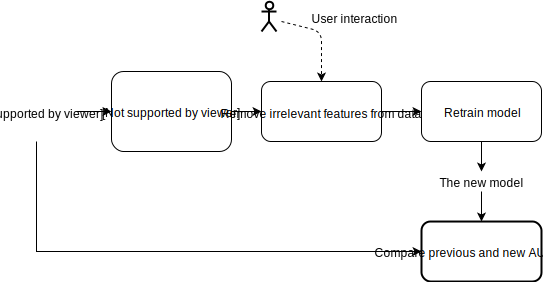
\includegraphics[scale=0.5]{img/method_schema.png}
    	\caption{Performance measure of an explanation algorithm. The performance is measured indirectly by how a user manages to improve a classifier.}
\end{figure}

To test the algorithm, two datasets are needed apart from the training set: 

\begin{itemize}
	\item A \textit{test dataset} in the same format as the train set --- That is: not cleaned from the untrustworthy features
	\item A \textit{validation dataset} that contains only the clean data with no irrelevant features.
\end{itemize}

The validation set is useful to test the generalizability of the model: if it performs well on both the test and the validation set, it is very generalizable. But if its score on the validation set is low, this is clearly not a good model. 

Hence, the baseline score of the model is its score on the \textit{validation set}: this is the score the model would obtain when applied on external data, it shows the ability for the model to generalize or not on new data. Meanwhile, the score on the unclean test set does not reflect the real performance of the model: this score should be probably higher than the one on the clean validation set. The higher the difference between these two score, the less trustworthy and generalizable the model is.

\section{Machine Learning models}

\subsection{Machine Learning estimators}

The purpose of this thesis is to find and test several algorithms that would have practical use at Dataiku and in the industry in general. This is why popular models will be tested: models that are widely used in production in many datascience projects.

Therefore two of the most used machine-learning models will be tested: \textit{logistic regression}, and \textit{Random Forests} \cite{Breiman2001}. Of course, if using model-independant explanations, any type of predictive model could be used, as long as it outputs either classification probability, or a regression prediction, like gradient boosted trees or neural networks for instance.

\subsection{Metrics}

The machine learning algorithms will be applied on test datasets to measure their performance. The logistic regression and random forests can output predicted probabilities, so the Reciever Operating Characteristics (ROC) will be used as a performance metrics on these algorithms. The algorithm score on a test dataset will therefore be the Area Under Curve (AUC) of the ROC curve.

Building a ROC curve consists in plotting the \textit{sensitivity} given the \textit{anti-specificity} of a binomial classifier. The sensitivity, also called true positive rate, is the rate of well-classified positive examples and the anti-specificity is the false positive rates, ie: the rate of negative examples marked as positive by the classifier. 

For a specific classifier that would predict directly the classes (0 and 1 for instance) and not probabilities for each class, the result would be a single point on the true-positive-rate versus false-positive-rate graph. But using classifiers that output probabilities, it is possible to use a moving threshold: examples predicted as positive can either be those with probability 0.8, 0.5, 0.3 or any value between 0 and 1. Therefore, the sensitivity and anti-specificity vary when this threshold is changed, which creates a set of point for a single classifier. Plotting these points creates a ROC curve.

The goal is to get closer to the perfect classifier that would have zero false-positive, and 100\% true-positives. This point is located at coordinates $(0, 1)$ on a ROC graph: therefore, we want the ROC curve to make the most acute angle it is possible near the point $(0,1)$.

\section{Algorithms tested}

As seen on Chapter 3 -- Background, this field of research led to many different algorithms that intend to explain machine learning models. In this thesis, a selection of algorithms will be tested, with several variants.

\subsection{Model-dependant}

As we will use either linear or tree-based models here, two kinds of model-dependant explanations will be used.

For linear models, the simple explanation algorithm relying on the linear coefficients and the features value, presented in Chapter 3, will be applied. The code has been implemented as a custom implementation for this thesis.

When testing tree-based models, Tree Interpreter will be used. It has been described in a blogpost \cite{treeinterpreter} and implemented on github by the blogpost author. An adaptation for gradient boosted trees made by the author of this thesis may also be used.

\subsection{Model-independent}

Among the large choice of model-independent explanations algorithms, two of them will be tested: \textit{Lime} \cite{lime}, and the Parzen-window-based \textit{explanation vectors} \cite{explvect}.

These algorithms are the most recent and above all: the fastest regarding computation time. Computing explanations for an individual example should be something fast enough: a user does certainly not want to wait 2 minutes to get an insight about an \textit{single} prediction, a few seconds is a maximum. Moreover, a high computation time makes it much harder to compute explanations for a large number of examples.

\section{Datasets}

The various methods will be tested on two different datasets. The Titanic dataset will be used to test the algorithms on a classical classification dataset. Some algorithms will also be applied on textual data --- a subset of the 20 news groups dataset.

The goal of the experiments is here to simulate a situation where there are many noisy features in the data, but the user cannot process them manually due to the high number of features. This situation would seem a bit artificial with these datasets, as the noisy/irrelevant features could actually be removed by an algorithm. But this is due to the evaluation method of the explanation algorithms.

Hence, the user will only remove the retrieved feature above a certain threshold: for the Titanic dataset, an irrelevant feature is removed only if it is in the top 3 influential feature for a given prediction. This simulates a situation where the user cannot access all the features in the same time.

\subsection{The Titanic dataset}

The well-known Titanic dataset will be reduced to its numerical columns. This dataset consists on the list of the Titanic passengers with several information provided on them. The set contains the information about the passenger, and the goal of the model is to predict whether a given individual survived or not the tragedy. Probabilistic algorithms actually predict the chances of survival for people on the test dataset rather than the death or survival.

Here we will be using a subset of the features: the passenger's age, sex, the ticket fare, the number of parents or children aboard, the number of spouses or siblings aboard. The passenger class is also used as a binary variable: 1 if the passenger travels in class 1 or 2, 0 for class 3. This makes a total of 6 variables.

As stated in section 3.5.1, the subset of the Titanic dataset that will be used here contains six numerical variables. All of them are meaningful and actually represent a Titanic passenger. Therefore, to this set of variables, a series of 8 meaningless variables will be added. These new variables consist in combinations of the 6 original variables, like age times ticket fare, age times passenger class, sex plus class, etc. To these combinations a random Gaussian noise is added. This creates correlation between variables, without them to have a real meaning in the dataset.

These features are added to the set of variables to form this 14-variable dataset.

The set is split into a train dataset, and test set and a clean validation set. For this last set, all the 8 meaningful variables have the same value for all the observations: these variables are all set to zero. There are 750 examples on the train set, 100 in the test dataset and 100 in the validation set.

\subsection{The 20 Newsgroups dataset}

The method will also be tested on part of the 20 News Groups Dataset. It consists on around 20,000 newsgroup documents, split into 20 different groups. In this dataset, we will only be using two classes: \textit{alt.atheism} and \textit{soc.religion.christian}. The classification problem becomes binary: is the posting user talking about atheism or Christianity. 

This dataset is interesting for several reasons: it is textual data, meaning the dimensionality is high. And above all, the data is very noisy: the data is e-mail-formatted text, with their headers and quotations from previous messages embedded. Therefore, it is very likely that a classifier would partly rely on wrong features, such as words in the header or e-mail addresses and not the actual text.

An example in this dataset will look like this:
\begin{center}
\begin{verbatim}
From: jonh@david.wheaton.edu (Jonathan Hayward)
Subject: Re: Pantheism & Environmentalism
Organization: Wheaton College, IL
Lines: 46

In article <Apr.5.23.31.36.1993.23919@athos.rutgers.edu> by028@cleveland.freenet.edu (Gary V. Cavano) writes:
>I'm new to this group, and maybe this has been covered already,
>but does anybody out there see the current emphasis on the
>environment being turned (unintentionally, of course) into
>pantheism?

Yes.
(I am adamantly an environmentalist.  I will not use styrofoam table service.
Please keep that in mind as you read this post - I do not wish to attack
environmentalism)
[...]
\end{verbatim}
\end{center}

To build the initial classifier, the process will be the following: compute the \textit{Term Frequencies-Inverse Document Frequencies} (Tf-Idf) of the corpus, and train a machine learning algorithm on the Tf-Idf. Then the user observes a series of examples and their explanations. The irrelevant words that show up in the explanation --- in the top 10 influential words --- such as words from the header, are removed, Tf-Idf is recomputed and a new model is trained.

The models are applied on both the test set, and the clean validation set for which the email headers and the quotes have been removed. A good algorithm should generalize well on the validation set, and scores on the test set and the validation set should be close. Of course, having removed the headers (that bring noise into the data) only on the validation set, we expect the scores to be different.


\chapter{Experiments}

Two similar experiments will be performed on two different datasets. The goal of the various explanation algorithms will be to find in the set of features the ones that are not meaningful in the data. Training again a new model on the new set of features should increase the score. Explanation algorithms will be judged given this increase of the score.

The initial dataset will therefore contain \textit{good} and \textit{bad} variables, meaning that some features should have a real meaning, while some other are falsely correlated to the target. Outputs of the explanations for a given prediction are presented to a human user, that will see which features are the most influential to the prediction. The user then decides to remove the meaningless features that are influential, hoping that removing these false correlations will increase the generalizability of the model.

To test this generalizability, there will be two datasets: one test dataset, similar to the train set, and one validation set that does not contain the meaningless features --- value zero is set for all these variables on this set. Therefore, a model that rely too much on these variables should perform badly on this validation dataset.

\section{20 news groups and Random Forest}

For the first experiment on the 20 newsgroups dataset, a Random Forest will be used as the machine learning algorithm over the Tf-Idf-transformed data. The ROC curves that are obtained when scoring the model on the test dataset and the clean validation dataset are plotted on figure 4.2.

Note that due to training time, it was not possible to compute explanations using the explanation vectors algorithm for this data set. The sampling process was simply taking too long, due to complexity issues and the large number of features: there are around 19000 different terms in this dataset.

\begin{figure}[h!]
		\centering
    	\def\svgwidth{\columnwidth}
    	\resizebox{0.75\textwidth}{!}{\input{img/roc-1.pdf_tex}}
    	\caption{Roc curve on the noisy test dataset (\textit{blue}, Area under curve: 0.986) and on the clean validation set (\textit{green}, AUC: 0.870)}
\end{figure}

As expected, there is a large difference between the score on the test set, that features the headers and previous messages quotations, and the validation set, cleaned from these noisy parts. These ROC curves mean that the model generalize badly on clean data: the model has learn noisy features from the presence of meaningless terms in the training set.

The goal now is to build a new model, starting from this bad one, using insights given by explanation algorithms. The explanations should contain features on which the model relies the most. Removing the features that the user considers as bad should improve the algorithm.

Below are the results for the three kinds of explanations algorithms tested. 20 examples from the test dataset are shown to the user, who then removes the meaningless features. These 20 examples are the same in the three methods.

\subsection{Treeinterpreter}

Treeinterpreter inspects the split in all the trees of a forest to compute the influence of each variable, as explained in the \textit{Background} section.

Here is an example of the explanation of one example made by treeinterpreter:

\begin{figure}[!h]
	\centering
   	\def\svgwidth{\columnwidth}
	\includegraphics[scale=0.35]{img/tree_interpreter.pdf}
    \caption{Output of \textit{treeinterpreter} on one example}
\end{figure}

We clearly see that many terms are only part of the e-mail header, and not real content written by the author of the message. Here the user's e-mail address provider is \texttt{@athos.rudgers.com}, an undergraduate school in New Jersey. The e-mail address was probably extracted from the header, and strongly associated with one class as this user may have posted a lot of messages.

Yet we do not want the classifier to rely on such features as they are only correlated with one of the classes on this small dataset: based on such features, a model would never generalize on new unseen data.

\begin{figure}[h!]
		\centering
    	\def\svgwidth{\columnwidth}
    	\resizebox{0.6\textwidth}{!}{\input{img/roc-treeinterpreter.pdf_tex}}
    	\caption{Roc curve on the noisy test dataset (\textit{blue}, AUC score: 0.972) and on the clean validation set (\textit{green}, AUC score: 0.890) after removing words using \textit{TreeInterpreter}.}
\end{figure}

After observing 20 messages from the test set, along with the model predictions and the explanations, the human user decides to remove the following terms from the training data:

\begin{center}
\begin{verbatim}
may, com, 1993, nntp, posting, re, co, gmt, ny, host, rutgers, 
article, edu, okcforum, ma, uk, tm, cu, 2000, writes, apr, clh, 
uga, wrote, inc, schneider, caltech, distribution, clh, cco, de, 
faq, clh, bil
\end{verbatim}
\end{center}

After retraining a new classifier on the new documents where the above words have been removed, the model slightly better: now the AUC on the clean validation dataset is 0.890, which is a better than the previous AUC on this set without removing any word --- 0.870, see previous section. Figure 4.3 presents the resulting ROC AUC. We can also note that the score on the noisy test dataset decreases, as features are removed. This was expected, and the real goal is to increase the score on the validation set, so such a decrease is not a problem at all.

Of course the score on the test set decreases, as the number of features that are both in the train and test sets decreases.

But what is to be noted is the slight increase of the score on the validation set. This means that the models relies more on meaningful terms than before. The model can generalize more efficiently. 

\subsection{Lime}

Lime outputs the following dashboard, featuring the score of the model on this example, the words importance, and the text with important words highlighted.

\begin{figure}[!h]
	\centering
   	\def\svgwidth{\columnwidth}
	\includegraphics[scale=0.35]{img/lime-output.png}
    \caption{Example of output by Lime}
\end{figure}

According to Lime, the classifier clearly used several non-accurate words to classify this example, header words: \textit{Subject}, \textit{In article}, names: \textit{James}, \textit{Bill}, or just stop-words like \textit{you}, \textit{isn't}.

After a user is asked to watch a list of 20 examples and remove all the non-relevant words, the following list of word is build, to be removed from the original documents:

\begin{center}
\begin{verbatim}
saturn.wwc vice.ICO Beauchaine rutgers.edu .edu sgi Re
solntze edu Nntp Posting nih.gov writes rice.edu PSUVM re
athos.rutgers.edu Host bobbe@ Dwyer bil@ .com article
Distribution geneva.rutgers 1993 UUCP NNTP uk cmu umd.edu
okcforum Institute of Technology wrote
\end{verbatim}
\end{center}

Stop-words (\textit{the}, \textit{is}, \textit{a}, ...) are actually kept since they are also in the validation dataset. Words that are removed are words on which the original model relies, while being either on the header or any non-relevant part of the message.

When removing these words from the original dataset, the new model reaches the following scores:

\begin{figure}[h]
		\centering
    	\def\svgwidth{\columnwidth}
    	\resizebox{0.6\textwidth}{!}{\input{img/roc-lime.pdf_tex}}
    	\caption{Roc curve on the noisy test dataset (\textit{blue}, AUC score: 0.945) and on the clean validation set (\textit{green}, AUC score: 0.902)}
\end{figure}

Lime, as well as treeinterpreter, manages to increase the score on the validation set, which proves that the model is now more general than before. But here it can be noticed that the two score on the test and the validation sets get much closer: the high AUC on the test set was misleading before, as there were many correlations between non meaningful terms and the target. Therefore, removing these meaningful features decreases the abnormally high score on the test set. 

\section{20 news groups and a linear model}

The results of the previous section showed important progress in improving the Random Forest classifier. But very sparse data such as texts, linear models are often preferred: they train much faster, can handle the large number of features easier than tree methods, and usually give good results.

Let's train a logistic regression on the 20 news groups dataset. The model performs slightly better than the random forest on the validation set, without taking out any term in the training set. As pictured on figure 4.6, the AUC on the test dataset is 0.976 and 0.917 on the validation set.

\begin{figure}[h]
		\centering
    	\def\svgwidth{\columnwidth}
    	\resizebox{0.6\textwidth}{!}{\input{img/roc-lr.pdf_tex}}
    	\caption{Roc curve on the noisy test dataset (\textit{blue}, AUC score: 0.976) and on the clean validation set (\textit{green}, AUC score: 0.917)}
\end{figure}

On this model, two explanation algorithms can be used: the linear model explanations --- model dependant explanation described in section 2.1.1 --- and Lime again, which is model independant. Let's apply both and try to increase the validation score with a logistic regression.

\subsection{Lime on linear model}

Just like with a random forest, Lime can be applied on a logistic regression. The same process is applied here: 20 examples are shown to a human user, who decides to remove features that are meaningless for this application. So words that are inconsistent with the decision to classify a text in a category or another are removed.

The useless word list gathered from the 20 examples is the following: 

\begin{center}
\begin{verbatim}
ai uga Michael Covington uxa uiuc edu Steve writes mangoe 
umd Livesey cs NNTP Posting Host okcforum Bill psuvm psu 
wam livesey solntze wpd sgi com mathew mantis co uk Mantis
Newsreader UK Mussack
\end{verbatim}
\end{center}

After retraining a new model on the train set where those words have been removed, we reach the following score on the test and validation set: AUC is 0.989 on the test set, and 0.925 on the validation set. The corresponding ROC curves are plotted on figure 4.7.

\begin{figure}[h!]
		\centering
    	\def\svgwidth{\columnwidth}
    	\resizebox{0.6\textwidth}{!}{\input{img/roc-lime-lr.pdf_tex}}
    	\caption{Roc curve on the noisy test dataset (\textit{blue}, AUC score: 0.989) and on the clean validation set (\textit{green}, AUC score: 0.925)}
\end{figure}

Contrary to the random forest case, this small cleaning increased the score on the test set. This is probably due to the fact that at each split a decision tree relies on the best feature, while the logistic regression handles all the features at once. Therefore noisy correlations between some features and the target can lower the score.

The increase on the validation dataset is very small. Nevertheless, it did increase the score. Showing the user more examples could probably have a stronger impact: here only 33 words have been removed, while the total number of features is around $19,000$.

Let us compare Lime's performances with the model dependant explanation on linear models.

\subsection{Linear model dependant explanation}

This kind of explanation, described in section 2.1.1, can be seen as the naïve approach for explaining linear model outcomes. 

As a reminder for the reader: this method just computes the element-wise product between feature values of the example and the coefficients of the linear model. The model output is directly proportional to the sum of this product. So determining which features have been the most influential on the prediction can be viewed as knowing which features contributed the most to this sum.

After computing the influential features for the 20 examples presented to a human individual, the meaningless terms are removed. On figure 4.8, the ROC curve of the new trained model is displayed: AUC score is 0.988 on the test dataset, and 0.922 on the validation set.

\begin{figure}[h!]
		\centering
    	\def\svgwidth{\columnwidth}
    	\resizebox{0.6\textwidth}{!}{\input{img/roc-linear-expl-lr.pdf_tex}}
    	\caption{Roc curve on the noisy test dataset (\textit{blue}, AUC score: 0.988) and on the clean validation set (\textit{green}, AUC score: 0.924)}
\end{figure}

Here again, the increase of the score on the validation set is slight but substantial.

\section{Titanic dataset}

As explained in section 3.5.1, the set of variables that will be used consists in 6 numerical features from the Titanic dataset and 8 additional irrelevant variables. A Random Forest with 100 trees is trained on this set.

Four explanation algorithms are used here: Tree Interpreter, the explanation vectors, Lime with the quartile discretizer and Lime with the entropy discretizer.

Each explanation algorithm is applied on 20 examples. These examples are presented to the user that decide to remove the meaningless features when they have too much importance. As opposed to the last section, here the bad variables are explicit: they are the one added by combining the original variables. Therefore the user does not have to be very clever: this work can be automated. But this actually simulates a situation where the user have a background knowledge on the data but cannot go through all the variables and check them manually.

In the same way, the dataset is splitted into three parts: a training set, a test set and a validation set. The validation set is cleaned from the meaningless features: for these variables the observation is always zero.

The initial ROC curve of the random forest on the noisy test set and the validation set is drawn on figure 4.9. The AUC on the test set is 0.907 while on the validation set, it is 0.837. That means, like in the 20 news groups case, that the model relies somehow on the meaningless features: if this was not the case the scores on the test and validation set should be closer.

\begin{figure}[h!]
		\centering
    	\def\svgwidth{\columnwidth}
    	\resizebox{0.6\textwidth}{!}{\input{img/titanic-roc-rf.pdf_tex}}
    	\caption{Roc curve of the initial model on the noisy test dataset (\textit{blue}, AUC score: 0.907) and on the clean validation set (\textit{green}, AUC score: 0.837)}
\end{figure}

The user is presented with the explanations for 20 examples from the test set. For all these examples, it has been decided that if a meaningless features falls in the top 3 influential features on the prediction, it should be removed. This ensure that all the bad variables are not all removed, simulating the fact that the user cannot manually remove all the features at once. On the 20 examples, over the 8 added features, usually 3 or 4 fall in the top 3 and are removed.

After having removed the features, new random forests are trained with the same parameters. The results are presented on table 4.1.

\begin{table}[ht]
  \begin{tabular}{c|c}
		\pbox{0.5\textwidth}{
			\resizebox{0.5\textwidth}{!}{\input{img/titanic-roc-lime-quartiles.pdf_tex}} \\ 
			Lime - quartile discretizer \\
			\textit{AUC on test set: 0.891} \\
			\textit{AUC on validation set: 0.867} \\} &
			
		\pbox{0.5\textwidth}{
			\resizebox{0.5\textwidth}{!}{\input{img/titanic-roc-lime-entropy.pdf_tex}} \\
			Lime - entropy discretizer \\
			\textit{AUC on test set: 0.881} \\
			\textit{AUC on validation set: 0.868} \\} \\ \hline
			
		\pbox{0.5\textwidth}{
			\resizebox{0.5\textwidth}{!}{\input{img/titanic-roc-tree-interpreter.pdf_tex}} \\
			TreeInterpreter \\
			\textit{AUC on test set: 0.894} \\
			\textit{AUC on validation set: 0.854.} \\} &
			
		\pbox{0.5\textwidth}{
			\resizebox{0.5\textwidth}{!}{\input{img/titanic-roc-parzen.pdf_tex}} \\
			Explanation vectors \\
			\textit{AUC on test set: 0.905} \\
			\textit{AUC on validation set: 0.833.} \\}
	\end{tabular}
  \caption{Roc curves on new models trained after removing irrelevant features. The explanation algorithm used is indicated as well as the AUC of the new model on both test and validation set.}
\end{table}

It can be noted that the AUC are very close when using Lime, and that the ROC curves are the closest with the entropy discretizer. TreeInterpreter and the explanation vectors manage to reduce somehow the gap between the AUCs, but it keeps relatively important compared to the initial gap.

\chapter{Discussions and conclusion}

In this thesis, several explanation methods have been confronted to one another. This chapter summaries the obtained results. Advantages and limits of the tested explanation algorithms are then discusses, and several possible improvement and paths for further investigation are proposed.

\section{Results summary}

First, experiments on both the Titanic and the 20 Newsgroups dataset showed that removing meaningless features can greatly improve generalizability of a model. Having such results is quite interesting, but this was expected.

But what is at stake here is the way explanations algorithms can help users improving models. A model that manages to output a influential meaningless feature provides valuable information. Therefore, good explanation algorithms are those that makes it easier for users to spot bad features among the most influential ones: these are the features that are the most likely to introduce noise in the model.

Table 5.1 is a summary of the increase of score of the model after having removed the influential bad features on the 20 newsgroups dataset. The greater increase the better for each explanation algorithm.

\begin{table}[ht]
\centering
  \begin{tabular}{|r|c|c|}
  	  \hline
	 Model &  \cellcolor{Gray} Random Forest &  \cellcolor{Gray} Logistic Regression \\ \hline
	 Lime & 0.032 & 0.008 \\ \hline
	 TreeInterpreter & 0.020 & N/A \\ \hline
	 Linear explanation & N/A & 0.007 \\ \hline
	 Explanation vectors & \multicolumn{2}{c}{N/A - Too long to compute}
	 \\ \hline
  \end{tabular}
  \caption{Increase in AUC after having removed meaningless features using a given explanation algorithm.}
\end{table}

On this dataset, Lime performs better than TreeInterpreter and the simple Linear interpreter, though the difference on the linear model is not really significant.

On the Titanic dataset, all the explanation algorithms are applied on a Random Forest's predictions. Table ... 

\begin{table}[ht]
\centering
  \begin{tabular}{|r|c|}
  	  \hline
	 Model &  \cellcolor{Gray} Random Forest \\ \hline
	 Lime - quartiles discretizer & 0.030\\ \hline
	 Lime - entropy discretizer & 0.031\\ \hline
	 Tree interpreter & 0.016\\ \hline
	 Explanation vectors & $-0.04$\\ \hline
  \end{tabular}
  \caption{Increase in AUC after having removed meaningless features using a given explanation algorithm.}
\end{table}

Here again, Lime is the most efficient in spotting the most influential features. It makes it easier for the user to remove the worthless influential variables from the data. TreeInterpreter performs quite well too. The explanation vectors, albeit looking promising on paper, do not get really interesting in practise. This limitation is discussed in section 5.2.

Overall, among all the algorithms tested, Lime seems to be the better: it spots the influential features for each prediction efficiently compared to the others. Moreover, computation is often fast, and can be speeded up by reducing the number of samples --- of course, this reduces its performances at some point.

The supervized binning based on entropy has similar results than using the quartiles as discretization method. These datasets are probably not the best one to show any improvement by the entropy binning. But, as stated in section  2.2.1, some improvement has been noticed on very skewed data.

\section{Limitations}

Despite providing valuable information about predictions to users, these methods suffer from several limitations. These limitations are usually different for each algorithm, so one should ponder over what is expected from the explanations, and which constraints are present.

\vspace{1em}

On TreeInterpreter and the Linear explanations, the main limitation is due to their model-dependant nature: these algorithms rely on the architecture of the machine learning model they try to explain. Therefore, they can only be used on one type of model, namely tree based models or linear models.

Moreover, when analysing classification and decision trees, it is not easy to get insights on how will behave the model when moving some feature values. Therefore, one cannot easily know if increasing a feature would increase or decrease the model output. This kind of information remains important in many cases where the list of influential alone is not sufficient: for instance, in a predictive maintenance context, a manager probably wants to know how each variable should be changed to reduce the costs.

\vspace{1em}

Model independent algorithms, on the contrary, are applicable to any machine learning algorithm, which is a great strength. Their explanations throughout models can be compared, because they have been computed the same way. Yet they also have some limitations.

Among the two model-independent algorithms tested, their main limitation is computation time. Lime is quite fast when computing predictions on one single example, but significantly slower than model dependant explanations. Usually, this does not let the user compute explanations for a large part of the data. Moreover, when dealing with a very large number of features, it is likely that the number of samples should be increased, which makes the computation longer.

Lime:
- not great on every point --> outliers

explanation vectors:
- speed
- not great on every point --> outliers
- sampling process

\section{Future work}

prout

\section{Conclusion}

:)


\nocite{mythos}
\nocite{euregulation}
\nocite{healthcare}
\nocite{trust}
\nocite{explainingclassif}
\nocite{evolutionnary}
\nocite{breastcancer}
\nocite{sensitivity}

\printbibliography

\end{document}
\endinput